% Source for schema.png, drawn from dutch_railway/dags/etl/sql/schema.sql.
% Rebuild from dutch_railway-docs/figures/ with:
%   pdflatex schema.tex && pdftoppm -png -r 600 -singlefile schema.pdf schema
\documentclass[tikz, border=4pt]{standalone}
\usepackage[T1]{fontenc}
\usepackage{lmodern}
\usetikzlibrary{shapes.multipart, positioning, calc}

\definecolor{accent}{HTML}{2F5D8C}
\definecolor{dimhead}{HTML}{DCE6F1}
\definecolor{note}{HTML}{555555}
\definecolor{keybg}{HTML}{F4F7FA}

% One column row: key marker, column name, type.
\newcommand{\col}[3]{\makebox[5mm][l]{\tiny\bfseries\color{accent}#1}\makebox[27mm][l]{\ttfamily #2}\makebox[13mm][r]{\tiny\color{note}#3}}
\newcommand{\head}[2]{\makebox[45mm][c]{\bfseries\color{#1}\ttfamily #2}}

\begin{document}
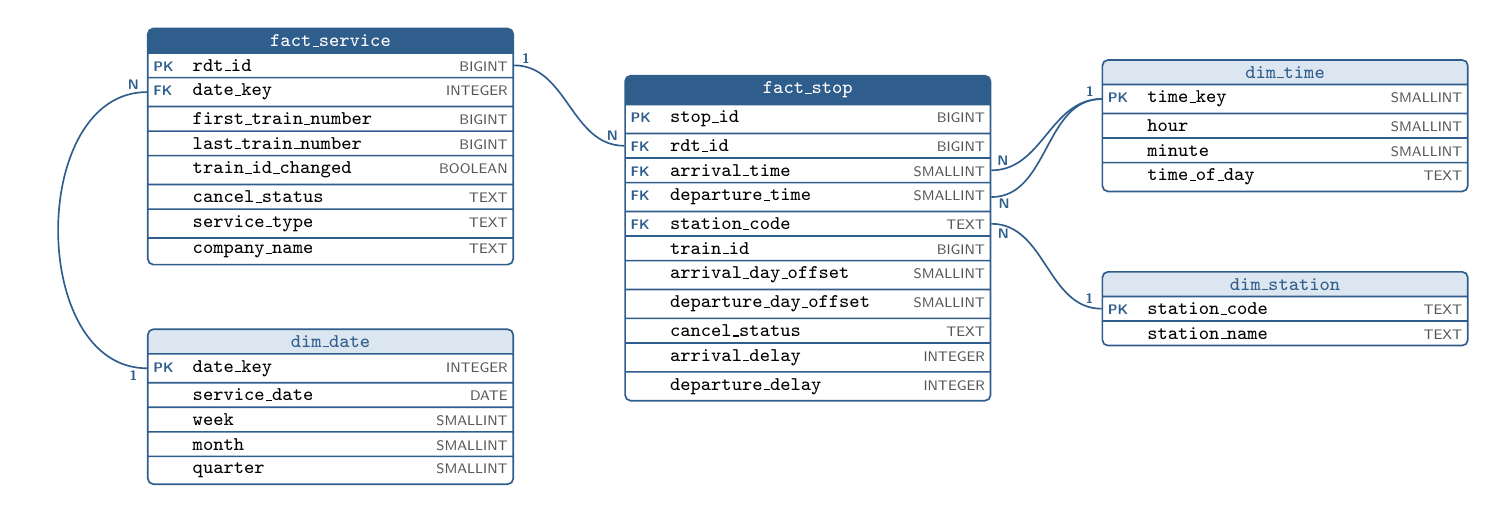
\begin{tikzpicture}[
    font=\sffamily\scriptsize,
    tbl/.style={rectangle split, rectangle split parts=#1, draw=accent, line width=0.6pt,
                rounded corners=2pt, inner sep=2pt, rectangle split part align=left},
    fact/.style={tbl=#1, rectangle split part fill={accent, white}},
    dim/.style={tbl=#1, rectangle split part fill={dimhead, white}},
    rel/.style={draw=accent, line width=0.6pt},
    card/.style={font=\sffamily\tiny\bfseries, text=accent, inner sep=1pt},
]

% Fact tables
\node[fact=9] (svc) at (0,0) {
  \head{white}{fact\_service}
  \nodepart{two}\col{PK}{rdt\_id}{BIGINT}
  \nodepart{three}\col{FK}{date\_key}{INTEGER}
  \nodepart{four}\col{}{first\_train\_number}{BIGINT}
  \nodepart{five}\col{}{last\_train\_number}{BIGINT}
  \nodepart{six}\col{}{train\_id\_changed}{BOOLEAN}
  \nodepart{seven}\col{}{cancel\_status}{TEXT}
  \nodepart{eight}\col{}{service\_type}{TEXT}
  \nodepart{nine}\col{}{company\_name}{TEXT}
};

\node[fact=12, anchor=north west] (stp) at ($(svc.north east)+(14mm,-6mm)$) {
  \head{white}{fact\_stop}
  \nodepart{two}\col{PK}{stop\_id}{BIGINT}
  \nodepart{three}\col{FK}{rdt\_id}{BIGINT}
  \nodepart{four}\col{FK}{arrival\_time}{SMALLINT}
  \nodepart{five}\col{FK}{departure\_time}{SMALLINT}
  \nodepart{six}\col{FK}{station\_code}{TEXT}
  \nodepart{seven}\col{}{train\_id}{BIGINT}
  \nodepart{eight}\col{}{arrival\_day\_offset}{SMALLINT}
  \nodepart{nine}\col{}{departure\_day\_offset}{SMALLINT}
  \nodepart{ten}\col{}{cancel\_status}{TEXT}
  \nodepart{eleven}\col{}{arrival\_delay}{INTEGER}
  \nodepart{twelve}\col{}{departure\_delay}{INTEGER}
};

% Dimension tables
\node[dim=6, anchor=north west] (date) at ($(svc.south west)+(0,-8mm)$) {
  \head{accent}{dim\_date}
  \nodepart{two}\col{PK}{date\_key}{INTEGER}
  \nodepart{three}\col{}{service\_date}{DATE}
  \nodepart{four}\col{}{week}{SMALLINT}
  \nodepart{five}\col{}{month}{SMALLINT}
  \nodepart{six}\col{}{quarter}{SMALLINT}
};

\node[dim=5, anchor=north west] (time) at ($(stp.north east)+(14mm,2mm)$) {
  \head{accent}{dim\_time}
  \nodepart{two}\col{PK}{time\_key}{SMALLINT}
  \nodepart{three}\col{}{hour}{SMALLINT}
  \nodepart{four}\col{}{minute}{SMALLINT}
  \nodepart{five}\col{}{time\_of\_day}{TEXT}
};

\node[dim=3, anchor=north west] (stn) at ($(time.south west)+(0,-10mm)$) {
  \head{accent}{dim\_station}
  \nodepart{two}\col{PK}{station\_code}{TEXT}
  \nodepart{three}\col{}{station\_name}{TEXT}
};

% Relationships: FK row (many) to PK row (one)
\draw[rel] (svc.three west) to[out=180, in=180, looseness=1.1]
  node[card, pos=0.04, above] {N} node[card, pos=0.96, below] {1} (date.two west);
\draw[rel] (stp.three west) to[out=180, in=0]
  node[card, pos=0.08, above] {N} node[card, pos=0.92, above] {1} (svc.two east);
\draw[rel] (stp.four east) to[out=0, in=180]
  node[card, pos=0.08, above] {N} node[card, pos=0.92, above] {1} (time.two west);
\draw[rel] (stp.five east) to[out=0, in=180]
  node[card, pos=0.08, below] {N} (time.two west);
\draw[rel] (stp.six east) to[out=0, in=180]
  node[card, pos=0.08, below] {N} node[card, pos=0.92, above] {1} (stn.two west);

\end{tikzpicture}
\end{document}
